\let\negmedspace\undefined
\let\negthickspace\undefined
\documentclass[journal]{IEEEtran}
\usepackage[a5paper, margin=10mm, onecolumn]{geometry}
%\usepackage{lmodern} % Ensure lmodern is loaded for pdflatex
\usepackage{tfrupee} % Include tfrupee package

\setlength{\headheight}{1cm} % Set the height of the header box
\setlength{\headsep}{0mm}     % Set the distance between the header box and the top of the text

\usepackage{gvv-book}
\usepackage{gvv}
\usepackage{cite}
\usepackage{amsmath,amssymb,amsfonts,amsthm}
\usepackage{algorithmic}
\usepackage{graphicx}
\usepackage{textcomp}
\usepackage{xcolor}
\usepackage{txfonts}
\usepackage{listings}
\usepackage{enumitem}
\usepackage{mathtools}
\usepackage{gensymb}
\usepackage{comment}
\usepackage[breaklinks=true]{hyperref}
\usepackage{tkz-euclide} 
\usepackage{listings}
% \usepackage{gvv}                                        
\def\inputGnumericTable{}                                 
\usepackage[latin1]{inputenc}                                
\usepackage{color}                                            
\usepackage{array}                                            
\usepackage{longtable}                                       
\usepackage{calc}  
\usepackage{amsmath,amssymb}

\usepackage{multicol}                                         
\usepackage{hhline}                                           
\usepackage{ifthen}                                           
\usepackage{lscape}
\begin{document}

\bibliographystyle{IEEEtran}

\title{
%	\logo{
NCERT - 10.3.6.1.1

\large{EE1003}
%	}
}
\author{Homa Harshitha Vuddanti

(EE24BTECH11062)
}	

\maketitle

\bigskip

\renewcommand{\thefigure}{\theenumi}
\renewcommand{\thetable}{\theenumi}
\textbf{Question}: Solve the pair of linear equations
\begin{align}
    \frac{1}{2x}+\frac{1}{3y}&=2\\
    \frac{1}{3x}+\frac{1}{2y}&=\frac{13}{6}
\end{align}\\
\textbf{Solution: }\\
Taking
\begin{align}
    \frac{1}{x}=u\\
    \frac{1}{y}=v
\end{align}
We get the equations as
\begin{align}
    3u+2v=12\\
    2u+3v=13
\end{align}
Writing them in matrix form
\begin{align}
\myvec{3 & 2 \\2 & 3}
\myvec{u\\v}=\myvec{12 \\ 13}
\end{align}
\textbf{LU decomposition:}\\
For the system of linear equations $\vec{A}\vec{x}=\vec{b}$, if $\vec{A}$ is non-singular, we can decompose it as product $LU$ where $L$ is lower triangular matrix and $U$ is an upper triangular matrix.\\
The equation becomes 
\begin{align}
    \vec{LUx}=\vec{b} \label{eq:1}
\end{align}
Taking 
\begin{align}
    \vec{y}=\vec{Ux}
\end{align}
Substituting in \eqref{eq:1},
\begin{align}
    \vec{Ly}=\vec{b}
\end{align}
We solve for $y$ in $\vec{L}\vec{y}=\vec{b}$ and then solve for $\vec{x}$ in $\vec{U}\vec{x}=\vec{y}$\\
Applying LU decomposition to matrix A, \\
For each column $j \geq k$, the entries of $U$ in the $k$th row are updated as:
\begin{align}
    U_{k,j} = A_{k,j} - \sum_{m=1}^{k-1} L_{k,m}.U_{m,j},   \forall{j \geq k}
\end{align}
For each row $i > k$, the entries of $L$ in the $k$th column are updated as:
\begin{align}
    L_{j,k} = \frac{1}{U_{k,k}}\brak{A_{j,k} - \sum_{m=1}^{k-1}.U_{m,k}}, \forall{i>k}
\end{align}
We find $\vec{L}$ and $\vec{U}$ as follows:
\begin{align}
    \vec{L}=\myvec{1 & 0 \\ \frac{2}{3}&1}\\
    \vec{U}=\myvec{3 & 2\\0 & \frac{5}{3}}
\end{align}
Solving $\vec{Ly}=\vec{b}$ by forward substitution,
\begin{align}
    \myvec{1 & 0 \\ \frac{2}{3}&1}\myvec{y_1\\y_2}&=\myvec{12 \\ 13}\\
    y_1&=12\\
    y_2&=5\\
    y&=\myvec{12\\5}
\end{align}
Solving $\vec{Ux}=\vec{y}$
\begin{align}
    \myvec{3 & 2\\0 & \frac{5}{3}}\myvec{u\\v}&=\myvec{12\\5}\\
    v&=3\\
    u&=2
\end{align}
Hence, solution is
\begin{align}
    x=\frac{1}{u}=\frac{1}{2}\\
    y=\frac{1}{v}=\frac{1}{3}\\
    \myvec{x\\y}=\myvec{\frac{1}{2}\\\frac{1}{3}}
\end{align}
\textbf{Plotting:}\\
\begin{figure}[h!]
   \centering
   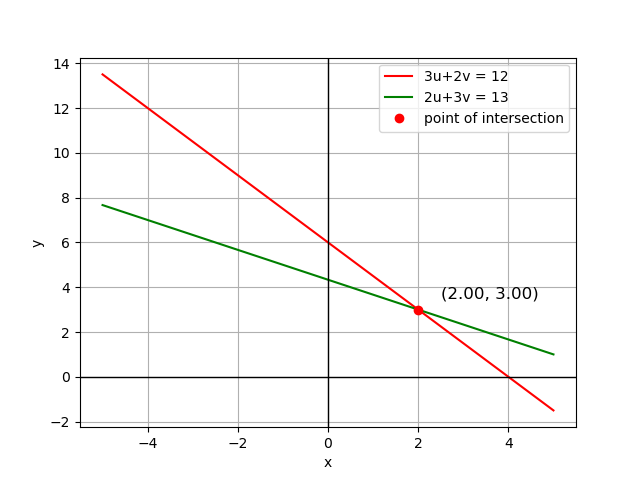
\includegraphics[width=1\columnwidth]{Figs/Figure_1.png}
   \caption{Plot}
\end{figure}
\end{document}





